\chapter{Background Theory and Related Work}

% THIS IS AN EXAMPLE. ALL SECTIONS BELOW ARE OPTIONAL. PLEASE CONSULT YOU ADVISOR AND DESIGN YOUR OWN SECTION

% \textthai{หัวข้อต่าง ๆ ในแต่ละบทเป็นเพียงตัวอย่างเท่านั้น หัวข้อที่จะใส่ในแต่ละบทขึ้นอยู่กับโปรเจคของนักศึกษาและอาจารย์ที่ปรึกษา}

% This is how you add the website URL: \url{http://www.cpe.kmutt.ac.th}

% Explain theory, algorithms, protocols, or existing research works and tools related to your work.

% You can cite your references like this: \cite{booch87}, or multiplie cite like this: \cite{meyer2000, atwoodmd}

This chapter outlines the theory and related research to ensure that the development is feasible and that there are appropriate tools. Relevant knowledge will be researched and summarized, along with the technologies and programming languages to be used. Additionally, competing solutions developed by others will also be discussed in this chapter.
\section{Background}
The Business Intelligence Infrastructure team at Agoda is responsible for assisting customers in retrieving data using SQL statements. Currently, 27\% of the tickets in BI-Help are categorized as 'Query Help.' This is because customers often struggle with writing SQL statements correctly, and SQL error messages can be difficult to understand. Additionally, with multiple databases, error messages can vary, and many users deal with highly complex SQL statements. Furthermore, other teams with limited SQL knowledge also seek assistance from the BI team to retrieve data from the database. To address these challenges, the team aims to develop Query Assistance to provide effective solutions.
\section{Theory and Core Concepts}
    \subsection{Large Language Models (LLMs)}
    Large Language Models are advanced AI systems designed to read and generate text based on their training from extensive datasets. Using deep learning techniques, they understand and process words and sentences. To enhance their responsiveness, LLMs undergo further fine-tuning. With additional training, these models can also be capable of translating languages.
    \subsection{Representational state transfer application programming interface (REST API)}
    Application Programming Interface (API) is middleware that facilitates communication between two software components. Representational State Transfer (REST) is a software architectural style that defines a set of constraints and principles on how an API should behave.
    \subsection{Software Architecture Pattern}
    Software architecture plays a crucial role in software development. It is a fundamental practice for developers to create software that is high-quality, efficient, and easy to manage and maintain. Software architecture consists of patterns that have been proven over time, becoming best practices that help solve common problems in software development. By following these patterns, developers can build systems that are easier to understand, maintain, and expand.
    
    These are the reasons why we need architectural patterns. First, software architecture acts as a visual communication tool, allowing other developers, colleagues, or even stakeholders to understand the system you are building in a much simpler way. Second, software architecture models make it easy to reuse them in other projects since you now know the decisions you made and the various trade-offs. Third, complex systems with many components and interactions need a clear structure to ensure everything works together smoothly. Fourth, systems expected to grow over time or handle high loads require careful planning to avoid bottlenecks and ensure they can scale efficiently. Fifth, long-term projects that will be developed and maintained over several years need a solid architectural foundation to prevent technical debt and ensure maintainability.
    \subsection{Multi Agent}
    \subsection{Performance Metrics}
\section{Languages and technologies}
    \subsection{Python}
    Python is a high-level programming language that serves multiple aspects of software development. Python offers a wide array of libraries that are invaluable for various tasks. For this project, we focus on utilizing Python to develop Large Language Models (LLMs).
    \subsection{LangChain}
    LangChain is a framework designed for building applications using Large Language Models. It streamlines the development process by enabling seamless transformation and integration of information through interconnected components.
    \subsection{Flask}
    Flask is a micro web framework for Python designed to enable the creation of lightweight and scalable web services. It offers simplicity and flexibility, making it an excellent choice for both small-scale applications and complex web services.
    \subsection{SQLAlchemy}
    SQLAlchemy is an SQL toolkit and Object Relational Mapper (ORM) for Python that assists in creating and managing relational databases. It provides a concise and efficient way to access and manipulate database data.
    \subsection{Alembic}
    Alembic is a lightweight database migration tool designed for use with SQLAlchemy. It helps ensure the consistency of the database schema by applying incremental changes in a controlled manner based on initial configuration settings.
    \subsection{Docker}
    Docker is a Container as a Service (CaaS) platform that is used to create isolated environments for running applications and storing data. It addresses hardware limitations and ensures consistent deployment across different environments.
    \subsection{GitLab CI}
    GitLab CI is a tool used for automation that works in coordination with GitLab to automate tasks such as testing, building, and deployment.
\section{Related research / Competing solutions}
    \subsection{SQLAI.ai}
    SQLAI.ai is a tool designed to assist with both SQL and NoSQL databases. It helps beginners learn SQL and allows SQL users to enhance their skills, accelerate their workflow, and optimize their queries. The tool was developed by a fast-moving startup based in Berlin, Germany, using GPT-4o as the AI model. There are seven features in this tool that assist users with both SQL and NoSQL, namely: generate SQL query, optimize SQL queries, fix SQL queries, explain SQL queries, simplify SQL query, format SQL query, and analyze your data. The tool supports 23 databases, including well-known ones such as MySQL, PostgreSQL, SQL Server (MS), Oracle PL/SQL, BigQuery, SQL, MariaDB, SQLite, MongoDB, DynamoDB, OrientDB, GraphQL, and Vertica. There are three ways users can obtain the database schema: by adding it manually with files, using AI to classify the file format and handle it automatically, or by connecting directly to the database. In terms of security, the tool limits the storage of sensitive data, e.g., it never stores actual database content. It only stores database schema (table and column names and data types) and credentials, which are fully encrypted. The actual database content is NEVER stored. Users can then choose the services they want to use.
    
    The scope of SQLAI.ai is significantly larger than the Query Assistance project. In terms of limitations, SQLAI.ai covers a broader area since it supports both SQL and NoSQL databases, 23 databases, and seven main features. There are three functions that both SQLAI.ai and Query Assistance share: generate SQL query, optimize SQL queries, and fix SQL queries. For fixing and optimizing SQL queries, SQLAI.ai provides more freedom for the user by offering a list of tailored fix suggestions for the SQL query. Users can choose the one they want to apply, and the AI will instantly generate a corrected query reflecting the applied step. Moreover, users can undo steps and view the differences between the original SQL query and the current one. On the other hand, Query Assist automatically fixes the SQL query and outputs only the corrected SQL query with some explanation. For generating SQL queries, both tools have similar features, but SQLAI.ai allows users to further adjust the query. Additionally, SQLAI.ai has an interface that, if the user is connected to a database, allows them to run queries directly by clicking the run button, displaying the results in a table, and generating an AI-created chart.

    
    \begin{table}[!h]
    \caption{test table method1}\label{tbl:method1}
        \begin{tabular}{c|c|l|rr} \hline\hline
            Center & Center & left aligned & Right & Right aligned \\ \hline\hline
            Center & Center & left aligned & Right & Right aligned \\ \hline
            Center & Center & left aligned & Right & Right aligned \\ 
            Center & Center & left aligned & Right & Right aligned \\ \hline
            Center & Center & left aligned & Right & Right aligned \\ \hline\hline
        \end{tabular}
    \end{table}

    You can place any report elements and refer to it like Figure~\ref{tbl:method1}, \ref{fig:oop-concept}
    The figure and table numbering will be run and updated automatically when you add/remove tables/figures from the document.

    \begin{figure}[H]
        \centering
        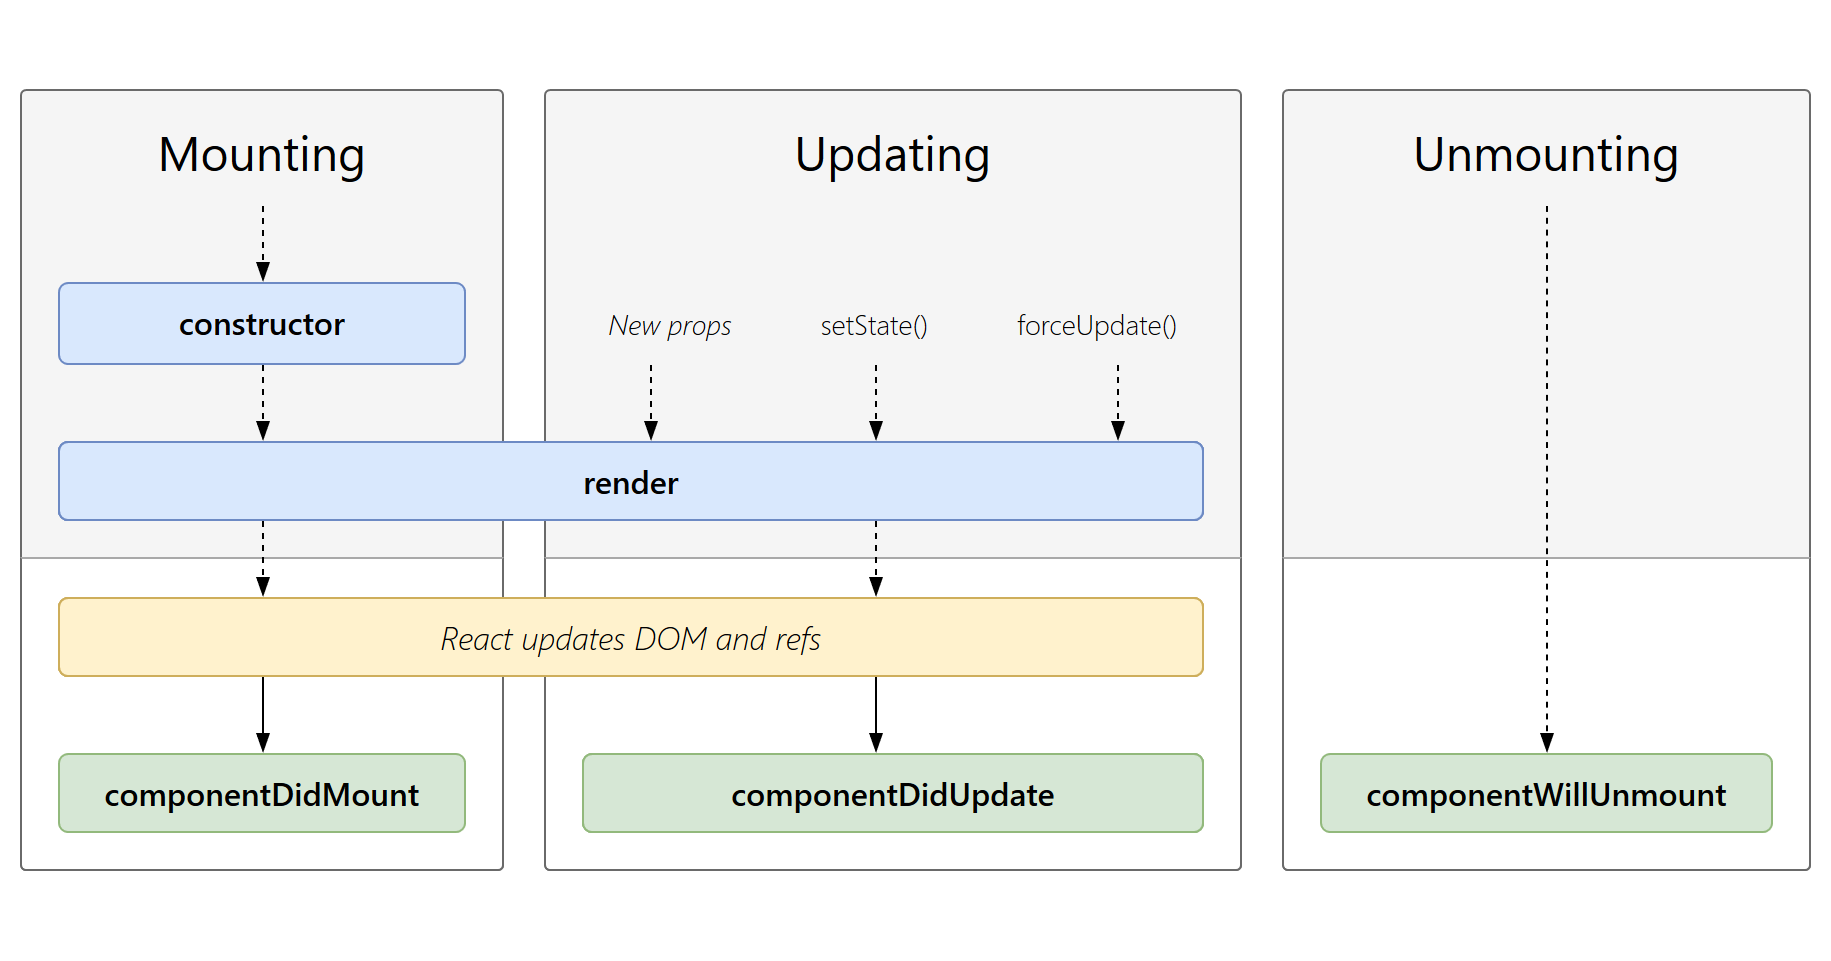
\includegraphics[width=7cm]{chapters/2/figures/react-lifecycle.png}
        \caption[Aspects of OOPs]{Aspects of OOPs from~\cite{apollo22oop}}
        \label{fig:oop-concept}
    \end{figure}
    
    \subsection{Algorithm I}
    Add more subsections as you want.
    \subsection{Algorithm II}
        Add more subsections as you want.
        \subsubsection{Step I}
            You can use subsection too!
        \subsubsection{Step II}
            This is the farthest level of subsection we permitted. (We support only 4th level)


\pagebreak